\chapter{State of the Art}
\label{chap:relatedwork}

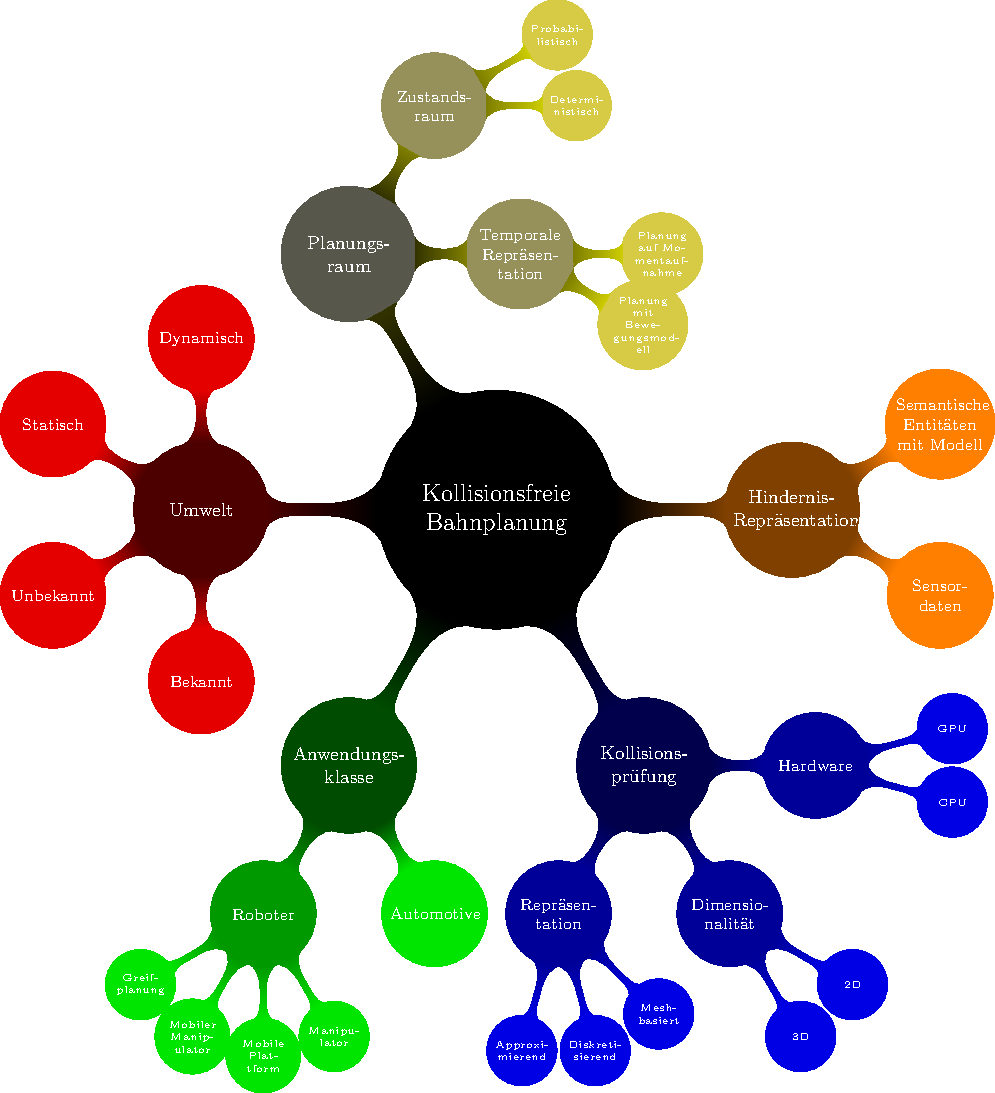
\includegraphics[width=1\textwidth]{04_images/sota_taxonomy}


Beispiel für ein ordinäres Zitat:~\cite{Schwarzer05adaptivedynamic}.

Beispiel für das Zitat einer eigenen Arbeit:~\citeownpubs{Hermann2014_ISR}.

Beispiel für das Zitat einer Studentischen Arbeit:~\citestudthesis{drews14}.

\section{General definition of corner cases}

See first PhD seminar
\begin{enumerate}
    \item rare event
    \item corner case
    \item edge case
    \item unusual event \cite{bolte_towards_2019}
    \item anomaly detection \cite{bolte_towards_2019}
    \item novelty detection \cite{bolte_towards_2019}
\end{enumerate}

\section{Definition of corner cases in the context of autonomous vehicles}

\todo{Knowledge-driven vs data-driven}

While the term \emph{corner case} is mentioned in the context of autonomous driving several times in the literature\todo[]{Find and cite literature before 2019}, no formal definition of its meaning was attempted until 2019, when Bolte et al. stated the following:

\begin{displayquote}[\cite{bolte_towards_2019}]
A corner case is given, if there is a non-predictable, 
relevant object/class in relevant location.
\end{displayquote}

This definition was motivated by the task of detecting corner cases in video data. Their proposed \emph{corner case detector} was designed as either an offline analysis tool for datasets or an online module to communicate corner cases to a \emph{autonomous driving system}.

Extended to Systemization by \cite{breitenstein_corner_2020, breitenstein_systematization_2020}

\begin{displayquote}[IESChat, Jasmin Breitenstein, 24 June 2021]
Wir haben die dann zusammen erweitert zu der Systematisierung, weil die bisherige Definition nicht alles abgebildet hat, vor allem nicht unser Bild, dass verschiedene Arten von CoCas verschiedene Detektionsmethoden brauchen
\end{displayquote}

Extended to typical AD-sensor stack (camera, radar, lidar) by \cite{heidecker_application-driven_2021}.

Different approaches from the same domain:

\begin{displayquote}[\cite{houben_inspect_2020}]
Inputs that result in unexpected or incorrect behaviour \end{displayquote}

\begin{displayquote}[\cite{hanhirova_machine_2020}]
Rare combinations of input parameter values \end{displayquote}

\begin{displayquote}[\cite{chou_using_2018}]
By an interesting corner case, we mean
initial conditions from which ensuring safety is hard but not
necessarily impossible 
\end{displayquote}

\begin{displayquote}[\cite{hesse_potenziale_2021}]
Trotzdem verbleibt ein Restrisiko für mögliches Fehlverhalten. Dieses tritt häufig im Zusammenhang mit sogenannten Edge und Corner Cases (Grenz- und Übergangsfälle) auf. Diese beschreiben Sonderfälle, die so selten auftreten, dass die Lernenden Systeme dafür gegebenenfalls nicht ausreichend konzipiert, trainiert und getestet wurden.
\end{displayquote}

Issue: Current cc detectors work with metric, so a system can known "that something is wrong" but it can hardly know "what is wrong". Therefore, machine-interpretable corner case description is necessary.

\section{Knowledge- and data-based descriptions of corner cases}

\section{Vision and multi-modal based detection of corner cases}

\section{Machine-learning based planning methods and their handling of corner cases}




